\section{Experiments}
\label{sec:experiments}

\subsection{Experiment Setup}
\label{sec:experiment_setup}

All experiments use a common pool of \num{10000} geographically distributed imaging requests sampled from populated places worldwide.
\figref{fig:worldcities_requests} shows the request distribution.
Each scheduling instance uses a \SI{24}{\hour} planning window and a circular \SI{400}{\kilo\metre} low-Earth orbit with the lookahead instrument configurations from \tabref{tab:lookahead_cases}.
Candidate lookahead observations are evaluated at their imaging time, so cloud state and insertion feasibility are tied to the actual acquisition epoch rather than to access-generation time.
Unless otherwise stated, the realistic-cloud experiments use the BCM clear probability prior $p=0.34$.

\begin{figure}[htbp]
    \centering
    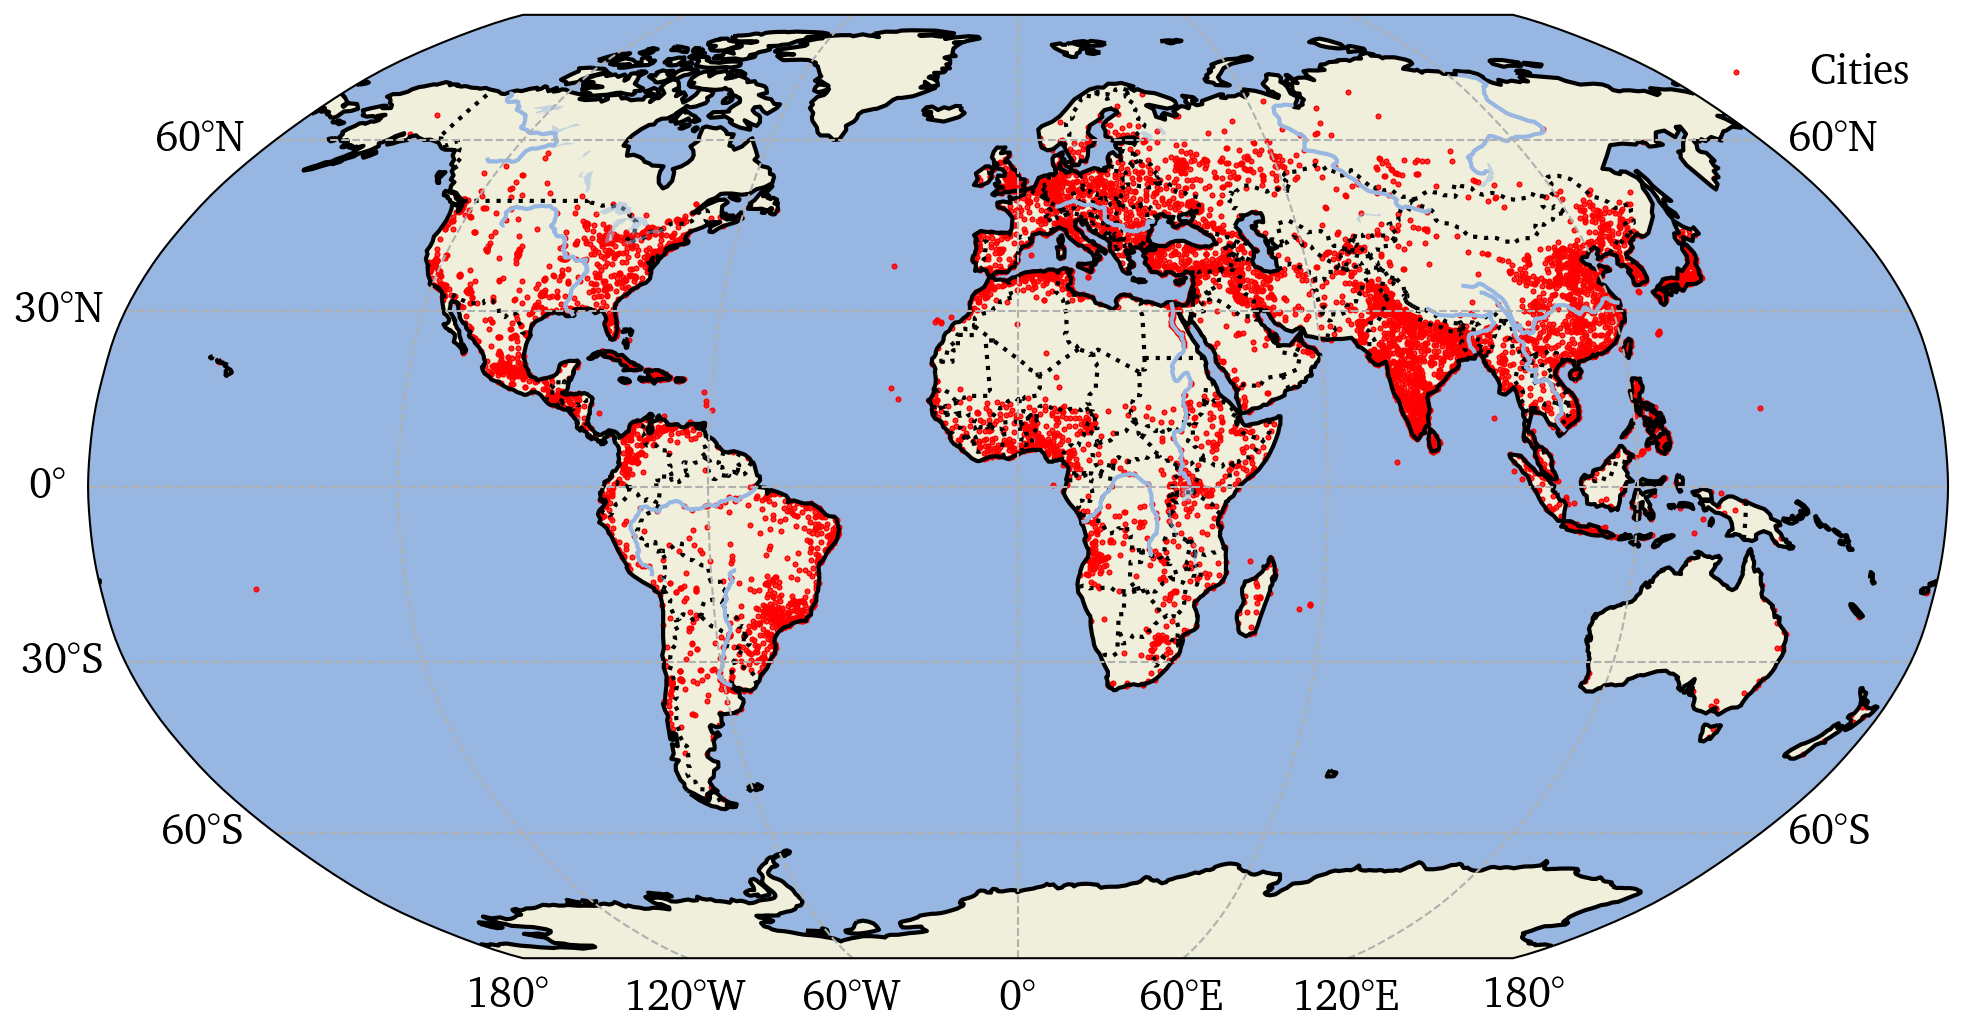
\includegraphics[width=0.72\linewidth]{figures/10k_worldcities.png}
    \caption{Global request set used for the scheduling experiments. The \num{10000} candidate targets are sampled from populated places, yielding dense coverage over major urban corridors while preserving worldwide geographic diversity.}
    \label{fig:worldcities_requests}
\end{figure}

\subsection{Experiment 1: Heuristic Calibration}
\label{sec:exp_heuristic_calibration}

This experiment calibrates the two-anchor value estimate and its break-even surrogate against paired Monte Carlo estimates of the true local insertion advantage in sampled iid repair windows.
The calibration separates the finite-window two-anchor value estimate $\widehat{K}_{2a}(g_{\mathrm{phys}})-B$ from its lightweight break-even surrogate $\widehat{K}_{b}(g_{\mathrm{phys}})-B$; $g_{\mathrm{break}}$ and $M=g_{\mathrm{break}}-g_{\mathrm{phys}}$ are retained as gate diagnostics rather than advantage estimators.
The sampler draws candidate density, cloud probability, physical spacing, and missed-task burden without conditioning on the sign of the heuristic, so the calibration includes both net-positive and net-negative lookahead windows.
For each sampled window, the Monte Carlo value is a conditional expectation over iid Bernoulli cloud states at the fixed candidate access times, not a full orbit-and-weather simulation.
In this iid setting the baseline term $B=p(N_{\mathrm{sched}}+N_{\mathrm{missed}})$ is unbiased by construction, so the residual bias after baseline subtraction reflects the chain approximation rather than the replacement-burden term.
The finite-window two-anchor estimator in \secref{sec:heuristic} removes this dominant boundary effect, while the break-even surrogate remains useful as a lightweight monotone onboard gate.
On the same anchor-normalized windows, the two-anchor advantage estimate attains CCC $0.992$ with bias $-0.025$, compared with CCC $0.982$ and bias $-0.305$ for the break-even surrogate.
All calibration panels report \SI{95}{\percent} bootstrap confidence intervals for CCC and bias, resampling windows while propagating the pointwise Monte Carlo standard error of each conditional mean; shaded bands show the corresponding \SI{95}{\percent} bootstrap confidence intervals for the least-squares calibration line.

\begin{figure}[htbp]
    \centering
    \begin{subfigure}[t]{0.48\linewidth}
        \centering
        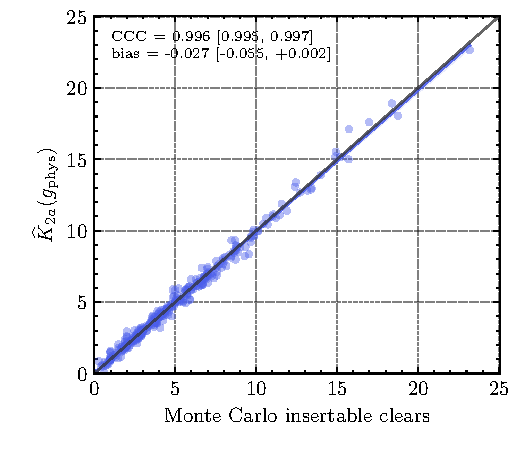
\includegraphics[width=\linewidth]{figures/two_anchor_calibration_chain.pdf}
        \caption{Two-anchor insertable clear-access count.}
        \label{fig:two_anchor_calibration_chain}
    \end{subfigure}
    \hfill
    \begin{subfigure}[t]{0.48\linewidth}
        \centering
        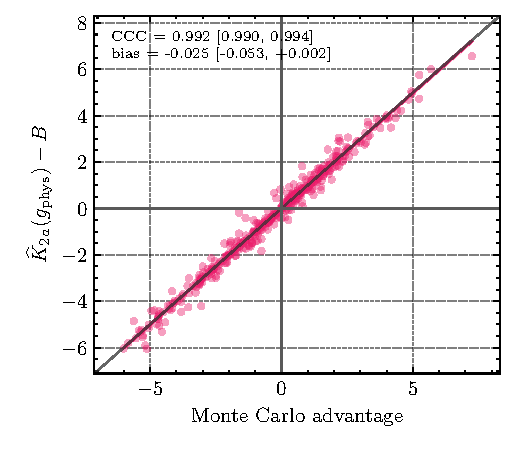
\includegraphics[width=\linewidth]{figures/two_anchor_calibration_advantage.pdf}
        \caption{Two-anchor net advantage.}
        \label{fig:two_anchor_calibration_advantage}
    \end{subfigure}
    \vspace{0.75em}
    \begin{subfigure}[t]{0.48\linewidth}
        \centering
        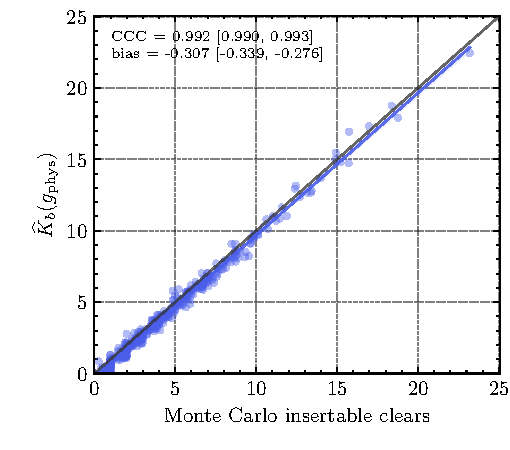
\includegraphics[width=\linewidth]{figures/breakeven_calibration_chain.pdf}
        \caption{Break-even insertable clear-access count.}
        \label{fig:breakeven_calibration_chain}
    \end{subfigure}
    \hfill
    \begin{subfigure}[t]{0.48\linewidth}
        \centering
        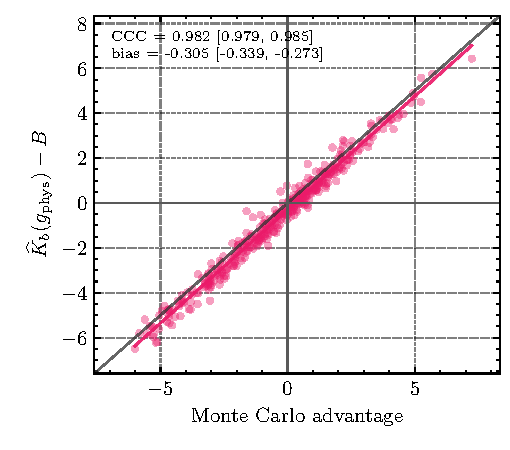
\includegraphics[width=\linewidth]{figures/breakeven_calibration_advantage.pdf}
        \caption{Break-even net advantage.}
        \label{fig:breakeven_calibration_advantage}
    \end{subfigure}
    \caption{Experiment~1 calibration on sampled iid repair windows. Each point fixes one synthetic window and reports the Monte Carlo mean over iid cloud-state draws. Panels compare the two-anchor estimate $\widehat{K}_{2a}(g_{\mathrm{phys}})$ and advantage $\widehat{K}_{2a}(g_{\mathrm{phys}})-B$ against the lightweight break-even surrogate $\widehat{K}_{b}(g_{\mathrm{phys}})$ and $\widehat{K}_{b}(g_{\mathrm{phys}})-B$.}
    \label{fig:heuristic_calibration_2x2}
\end{figure}

\begin{figure}[htbp]
    \centering
    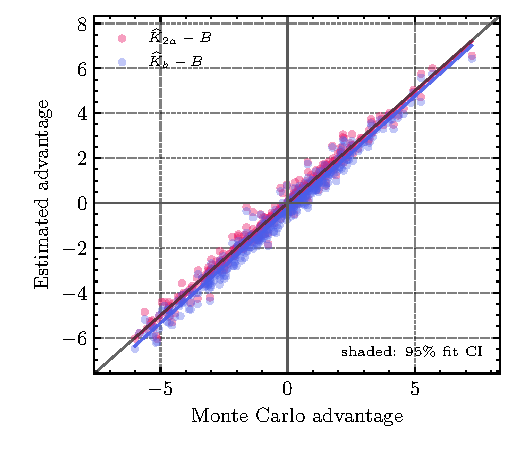
\includegraphics[width=0.5\linewidth]{figures/two_anchor_advantage_comparison.pdf}
    \caption{Direct comparison of the Experiment~1 advantage estimators. Candidate accesses are sampled on the full anchor interval $[t_L,t_R]$, while insertable clear chains must lie in the anchor-trimmed interval $[t_L+g,t_R-g]$. The two-anchor estimator closely tracks the Monte Carlo advantage, whereas the break-even surrogate $\widehat{K}_{b}$ is deliberately lightweight and slightly conservative on these windows. Shaded bands show \SI{95}{\percent} bootstrap confidence intervals for the least-squares calibration lines, including pointwise Monte Carlo standard error.}
    \label{fig:two_anchor_advantage_comparison}
\end{figure}
\FloatBarrier

\subsection{Experiment 2: IID End-to-End Scheduling}
\label{sec:exp_iid_scheduling}

This experiment evaluates greedy, break-even, and two-anchor policies inside the full receding-horizon scheduler under iid Bernoulli cloud truth.
Each trial constructs the conventional schedule, samples realized cloud states independently with $p_{\mathrm{clear}}=0.34$, computes an omniscient clear-sky upper bound, and then replays paired dynamic-tasking policies on the same access set and cloud realization.
To isolate the cloud model, the trial dates and RAAN phase matching are identical to the BCM case study in \secref{sec:exp_bcm_case_study}; only the cloud-state generator changes.
Across \num{12} paired \SI{24}{\hour} trials using the full \num{10000}-request pool, we sweep the two lookahead FoVs in \tabref{tab:lookahead_cases}, $\Theta_h=\Theta_v\in\{\ang{45},\ang{60}\}$, and three representative agility settings, $t_{\mathrm{slew}}(\theta_{\mathrm{FoR}})\in\{25,35,45\}$~s.
Each policy scores \num{64} candidate pitch angles per scheduling gap.
The two-anchor policy tests the finite-window estimator directly, while the break-even policy tests the monotone gate derived from $\widehat{K}_{b}$.
Across all FoV/agility cells, the value-based policies dominate the greedy baseline in gap closure while using about \SI{40}{\percent} fewer lookahead actions per scheduled access.
Averaged across the sweep, greedy closes \SI{51.3}{\percent} of the omniscient gap with 0.270 lookaheads per scheduled access.
The break-even gate closes \SI{72.1}{\percent} with 0.163 lookaheads per scheduled access, while the two-anchor policy closes \SI{72.8}{\percent} with 0.166.
The strongest cell is the \ang{60}$\times$\ang{60} lookahead FoV with $t_{\mathrm{slew}}(\theta_{\mathrm{FoR}})=\SI{45}{\second}$: break-even closes \SI{82.1}{\percent} of the gap with 0.200 lookaheads per scheduled access, and two-anchor closes \SI{81.9}{\percent} with 0.200.
\todo{Expand this interpretation: break-even and two-anchor are nearly indistinguishable in the iid end-to-end scheduler once the anchor-support correction is applied, so the final paper should decide whether to present break-even as the lightweight onboard rule and two-anchor as its finite-window justification.}
Detailed numerical summaries are reported in Appendix~\ref{sec:appendix_iid_scheduling_summary}.

\begin{figure}[H]
    \centering
    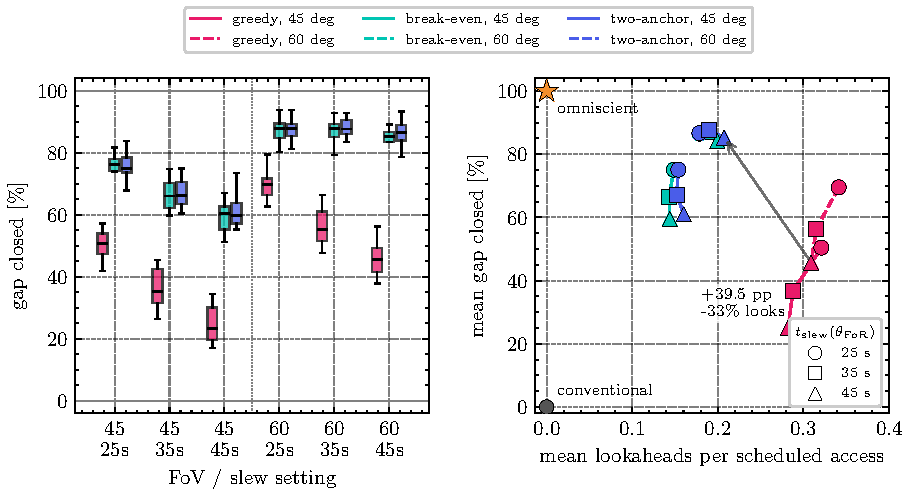
\includegraphics[width=0.92\linewidth]{figures/iid_scheduling_tradeoff.pdf}
    \caption{IID end-to-end scheduling over \num{12} paired \SI{24}{\hour} trials per FoV/agility cell. Left: per-trial distribution of the conventional-to-omniscient gap fraction closed. Right: mean gap closure versus mean lookaheads per scheduled access for the same FoV/agility cells; marker shape encodes agility. Solid lines use the \ang{45}$\times$\ang{45} lookahead FoV; dashed lines use the \ang{60}$\times$\ang{60} FoV. The gray dot and orange star mark the conventional and omniscient references.}
    \label{fig:iid_scheduling_tradeoff}
\end{figure}

\subsection{Experiment 3: Realistic BCM Case Study}
\label{sec:exp_bcm_case_study}

This experiment repeats the end-to-end scheduler sweep using realistic cloud truth from geostationary Binary Cloud Mask products.
We use \num{12} paired \SI{24}{\hour} windows spanning the available 2025 archive, with trial starts on Jan.~1, Feb.~2, Mar.~1, Apr.~1, May~1, Jun.~1, Jul.~1, Aug.~1, Sep.~1, Oct.~1, Oct.~10, and Dec.~1.
The February and late-year dates are shifted from exact month starts only to avoid verified source-product gaps in the GOES and Himawari archives.
For all date-based trials, the RAAN is phase-matched to the first window so that each trial repeats the same Earth-fixed ground track; remaining seasonal variation therefore comes from illumination and cloud structure rather than from a drifting target overpass pattern.
The policy prior remains fixed at $p_{\mathrm{clear}}=0.34$, while realized clear/cloudy states are sampled from the nearest available source product at each access imaging time.

\figref{fig:bcm_scheduling_tradeoff} shows that the value-based gates remain effective under spatially structured cloud fields.
Averaged across all six FoV/agility cells, the break-even gate closes \SI{70.1}{\percent} of the conventional-to-omniscient gap using 0.162 lookaheads per scheduled access, while the two-anchor gate closes \SI{71.8}{\percent} using 0.165 lookaheads per scheduled access.
The greedy baseline closes \SI{36.7}{\percent} on average but uses 0.264 lookaheads per scheduled access.
The strongest BCM setting is the \ang{60}$\times$\ang{60} lookahead FoV with $t_{\mathrm{slew}}(\theta_{\mathrm{FoR}})=\SI{45}{\second}$: break-even closes \SI{80.1}{\percent} of the gap with 0.196 lookaheads per scheduled access, and two-anchor closes \SI{81.3}{\percent} with 0.198.
With the anchor-consistent support definition, the two-anchor estimator and break-even surrogate now make similar operational decisions; two-anchor is slightly stronger on average in this sweep.
Detailed numerical summaries are reported in Appendix~\ref{sec:appendix_bcm_scheduling_summary}.

\begin{figure}[H]
    \centering
    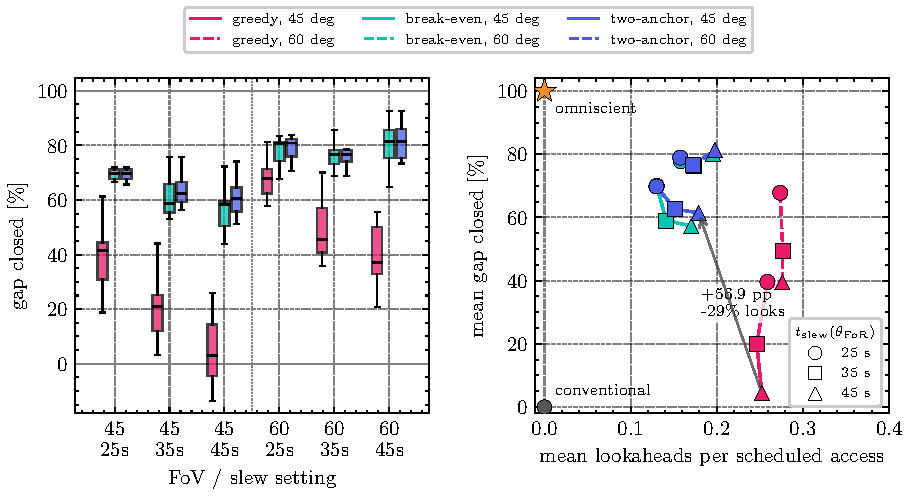
\includegraphics[width=0.92\linewidth]{figures/bcm_scheduling_tradeoff.pdf}
    \caption{BCM end-to-end scheduling over \num{12} paired \SI{24}{\hour} trials per FoV/agility cell. Trial RAAN is phase-matched across dates to preserve the Earth-fixed ground track while cloud truth is sampled from realistic geostationary cloud-mask products at each access imaging time. Left: per-trial distribution of the conventional-to-omniscient gap fraction closed. Right: mean gap closure versus mean lookaheads per scheduled access; marker shape encodes agility, line style encodes FoV, and the gray dot/orange star mark conventional and omniscient references.}
    \label{fig:bcm_scheduling_tradeoff}
\end{figure}

\subsection{Experiment 4: Overflight Case Study}
\label{sec:exp_overflight_case_study}

As a representative single-pass case study, \figref{fig:ma_overflight_case_study} compares the two value-based policies on the same Morocco-to-Australia overflight and iid cloud realization.
Both panels use the same access set, conventional schedule, and camera model; only the lookahead gate changes.
Break-even uses \num{11} lookaheads and two-anchor uses \num{14}, with both policies scheduling \num{48} clear images after local repair.

\begin{figure}[H]
    \centering
    \begin{subfigure}[t]{0.48\linewidth}
        \centering
        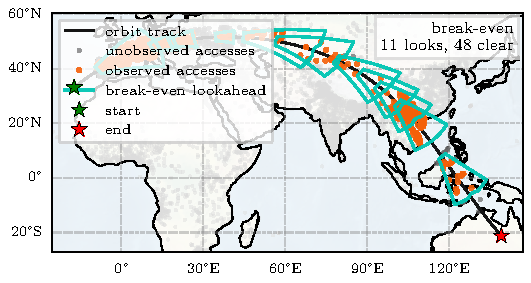
\includegraphics[width=\linewidth]{figures/lookahead_chain_ma_break_even.pdf}
        \caption{Break-even gate.}
        \label{fig:ma_overflight_break_even}
    \end{subfigure}
    \hfill
    \begin{subfigure}[t]{0.48\linewidth}
        \centering
        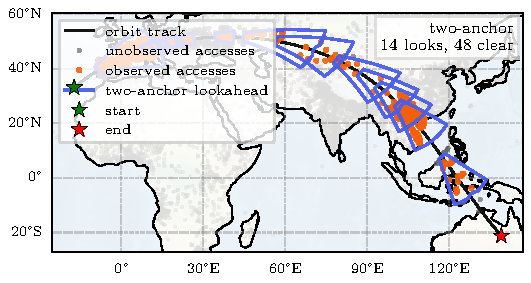
\includegraphics[width=\linewidth]{figures/lookahead_chain_ma_two_anchor.pdf}
        \caption{Two-anchor gate.}
        \label{fig:ma_overflight_two_anchor}
    \end{subfigure}
    \caption{Representative Morocco-to-Australia overflight case study. Orange dots mark accesses observed by the lookahead instrument, gray dots mark unobserved accesses, and colored outlines show the detector footprints selected by each policy.}
    \label{fig:ma_overflight_case_study}
\end{figure}

\figref{fig:brazil_overflight_case_study} shows the same comparison on the South America overpass used during development.
This case includes a zero-utility virtual anchor near the start of the pass so that the receding-horizon rule can evaluate the initial offshore reconnaissance gap before the first conventional imaging task.
With that anchor, both value gates take \num{6} lookaheads and schedule \num{23} clear images in the repaired pass.

\begin{figure}[H]
    \centering
    \begin{subfigure}[t]{0.48\linewidth}
        \centering
        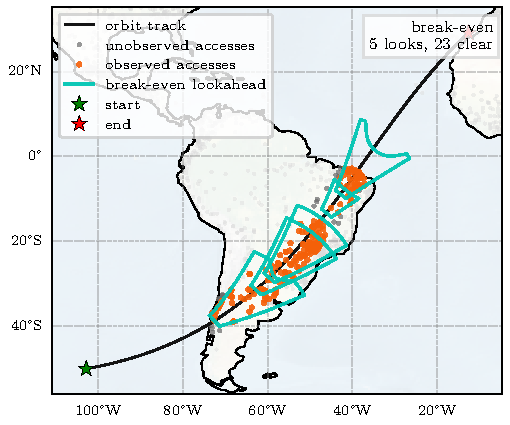
\includegraphics[width=\linewidth]{figures/lookahead_chain_brazil_break_even.pdf}
        \caption{Break-even gate.}
        \label{fig:brazil_overflight_break_even}
    \end{subfigure}
    \hfill
    \begin{subfigure}[t]{0.48\linewidth}
        \centering
        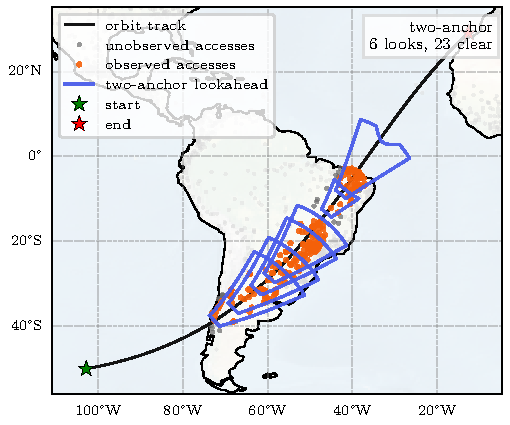
\includegraphics[width=\linewidth]{figures/lookahead_chain_brazil_two_anchor.pdf}
        \caption{Two-anchor gate.}
        \label{fig:brazil_overflight_two_anchor}
    \end{subfigure}
    \caption{Brazil overpass case study using the same visual encoding as \figref{fig:ma_overflight_case_study}.}
    \label{fig:brazil_overflight_case_study}
\end{figure}
